

\begin{document}\selectlanguage{ngerman}
\section*{LHCb und LHC}
\begin{figure}[h]
     \begin{minipage}[t]{0.6\textwidth}
      \vspace{-6cm} Wir kennen den Aufbau des LHCb-Detektors am CERN aus dem Einführungsvortrag. Nun wollen wir die Informationen nutzen und Teilchen untersuchen, die wir mit dem Detektor direkt messen können. Aus den Massen der gemessenen Teilchen kann anschließend die Masse des Mutterteilchens rekonstruiert werden, das werden wir heute Nachmittag sehen! 
      
      Wir nehmen den Detektor als zweidimensional an, sowie dass die Kalorimeter die Energie sehr exakt bestimmen können (s. Abb. \ref{fig: Der Detektor}). Dies hat den Vorteil, dass die RICH-Subdetektoren vernachlässigt werden können. Der Magnet wird als homogen angenommen. Konstanten: Vakuumlichtgeschwindigkeit $c~=~ 299792458 \, \nicefrac{m}{s}$; Elementarladung $e~=~ 1.602176634\cdot10^{-19}$\,C.  \end{minipage}
            \begin{minipage}[t]{0.4\textwidth}
            \centering
            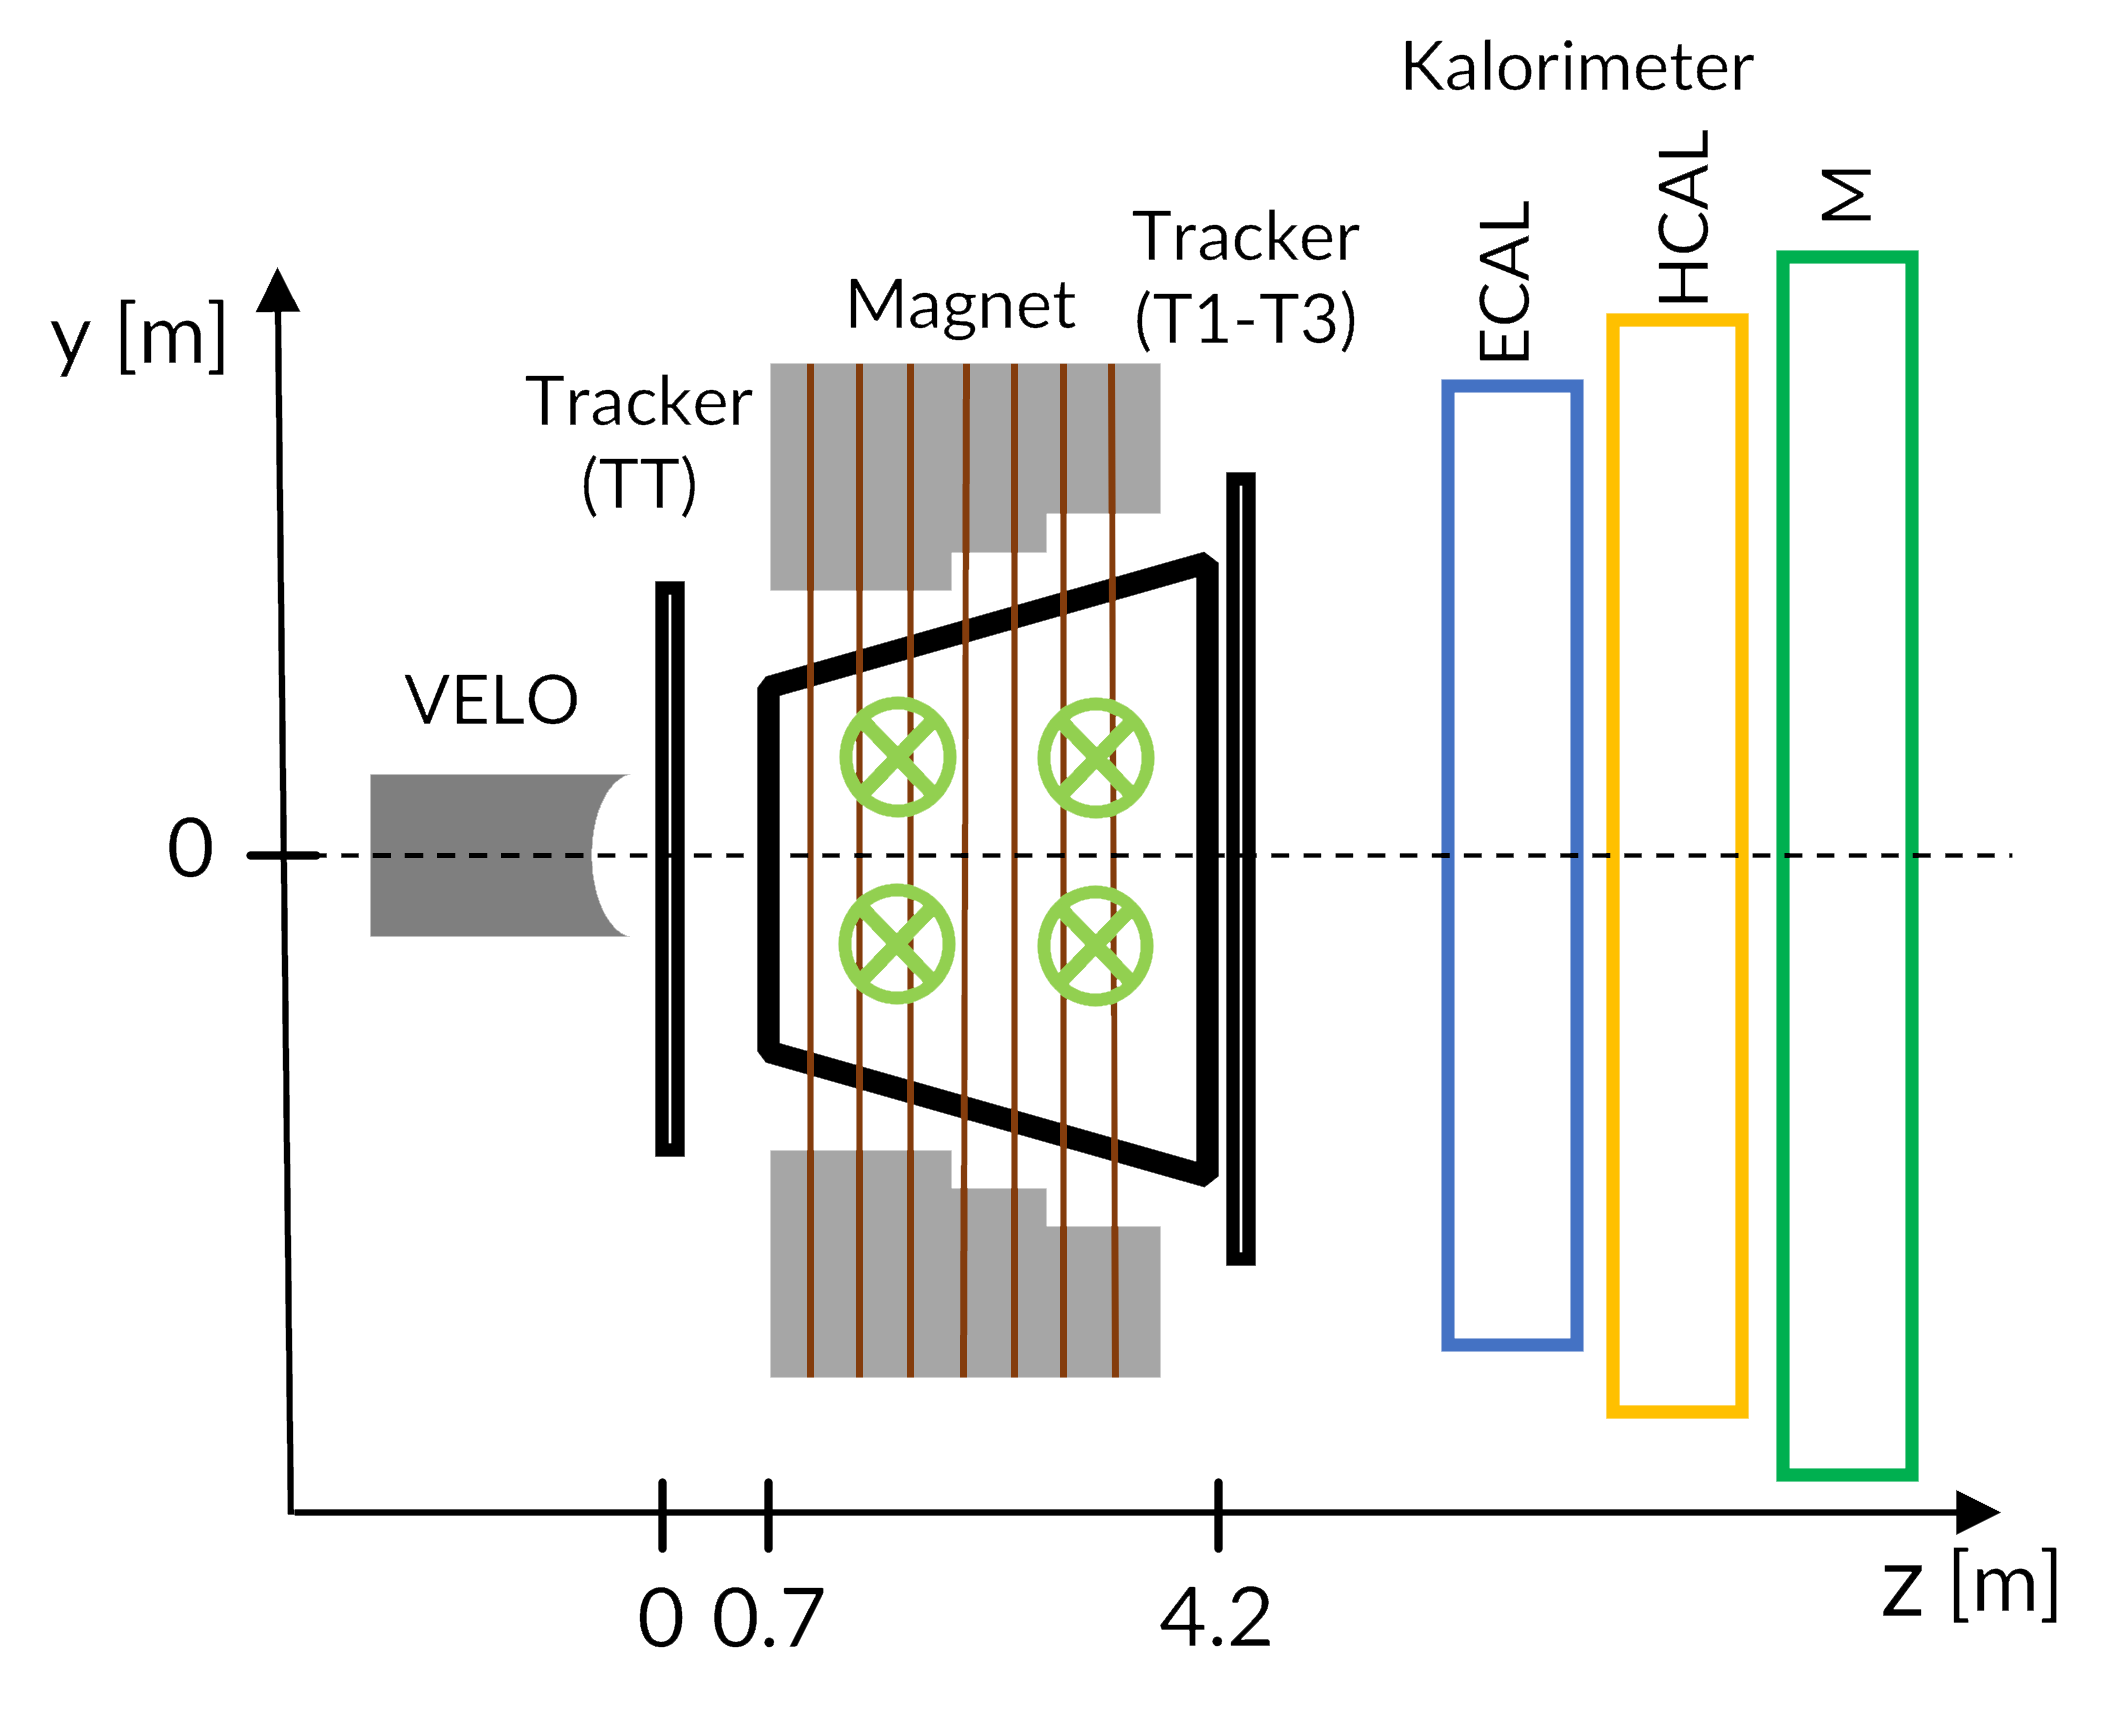
\includegraphics[width=\textwidth]{Figures Worksheets/LHCb_Calculation_LHCb_Detector_DE.png} 
            \caption{Vereinfachter LHCb-Detektor} \label{fig: Der Detektor}
            \end{minipage}
            \end{figure}
\subsection*{Messdaten}
Die nachstehende Tabelle beinhaltet die Daten eines Zerfalls, welcher das Triggersystem aktiviert und als womöglich spannend identifiziert hat. Außerdem sehen Sie einen Ausschnitt des Vertex Locators (VELO), welcher sich um den Kollisionspunkt befindet. Dort interagieren die Reaktionsprodukte mit hintereinander angeordneten Siliciummodulen  (grün), sodass sich Spuren und Ursprungspunkte sekundärer Zerfälle identifizieren lassen.
\begin{figure}[h]
    \centering
   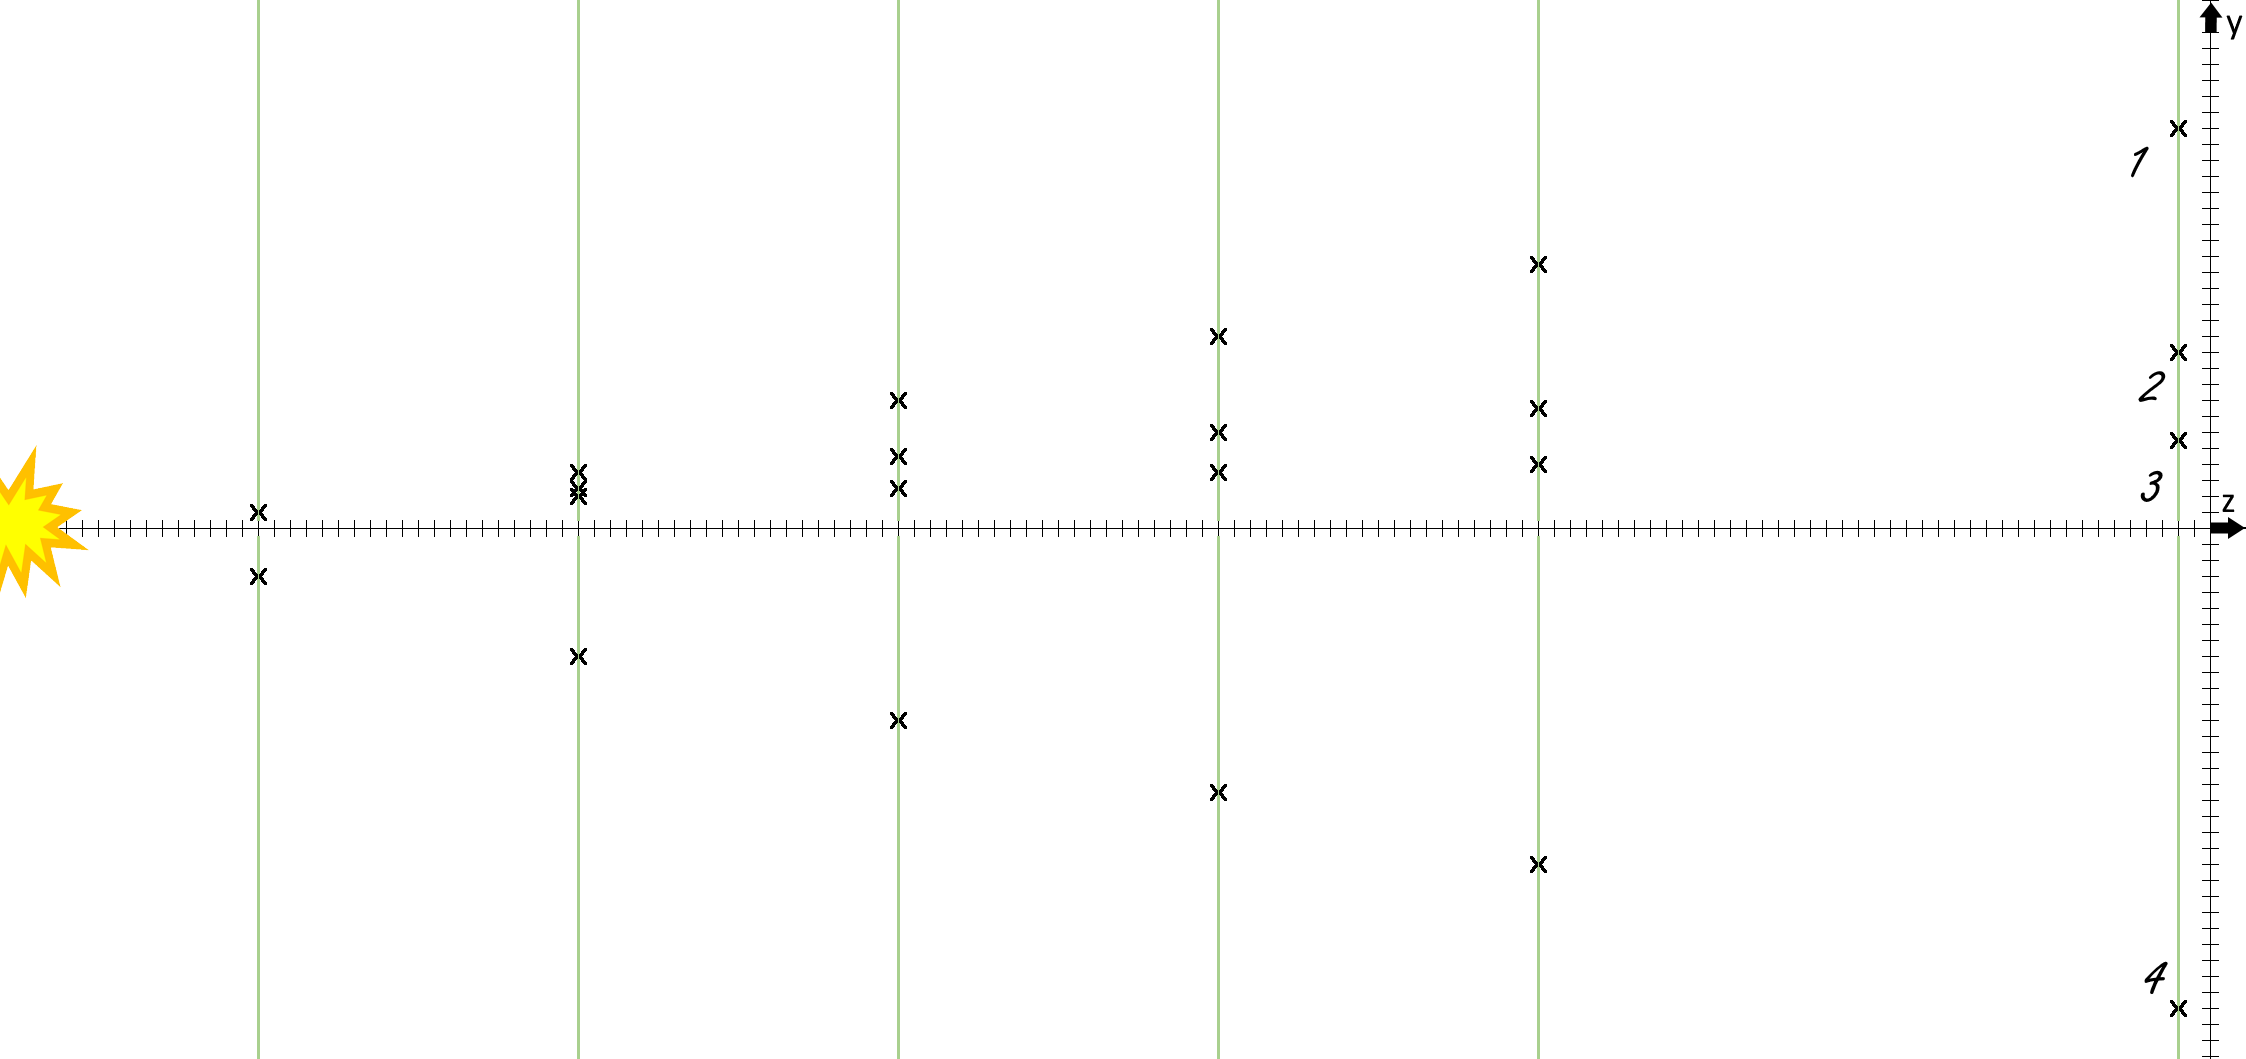
\includegraphics[width=\textwidth]{Figures Worksheets/LHCb_Calculation Task.png}\label{fig: VELO}
   \caption{Seitliche Ansicht der Ereignisse an den Siliciummodulen (grün) des VELOs, welcher um den Kollisionspunkt angeordnet ist. Hieraus lassen sich Ursprungsorte von weiteren Zerfällen und Winkel von Spuren relativ zur $z$-Achse bestimmen.}
\end{figure}
\begin{table}
\centering
 \caption{Datentabelle über das Ereignis. Angegeben für die Spuren die Orte im Trackersystem vor (TT) und nach (T1-T3) dem Magnetfeld. Die im Elektromagnetischen Kaloriemeter (ECAL) deponierte Energie sowie die im Hadronischen Kaloriemeter (HCAL) sind zu einer Gesamtenergie verrechnet worden. Außerdem die Angabe, ob das Myonensystem (M) getriggert wurde.}
\begin{tabular}{|r||r|r|r|r|c|}

\hline
\rowcolor{LHCbDarkBlue} \T\B \textcolor{LHCbLightBlue}{Spur} & \textcolor{LHCbLightBlue}{TT} & \textcolor{LHCbLightBlue}{T1-3} & \textcolor{LHCbLightBlue}{ECAL} & \textcolor{LHCbLightBlue}{HCAL} & \textcolor{LHCbLightBlue}{M}  \\
\hline\rowcolor{LHCbLightBlue}\T\B  & y/m & y/m & E/GeV & E/GeV & \\
\hline\hline 
\T\B 1 & 0.72769 & 2.89240 & 0.0461& 0.3727& Leer\\ 
\T\B 2 & 0.30505 & 0.83866 & 0.4902 & 3.9661 & Leer\\
\T\B 3 & 0.12215 & -0.02320 & 0.3072 & 2.2530 & Leer \\ 
\T\B 4 & -0.78733 & -1.93223 & 0.4791 & 3.5142 & Leer \\  


\hline
\end{tabular}\end{table}\\ \, \\ 
\kariert{Platz für Notizen und Zeichnungen}{17}{14}



\newpage



\SetDefinition{\textbf{Aufgabe 1:} Bilden Sie  Geraden aus den Messpunkten im VELO, s. Abb. 2. Diskutieren Sie Ihre Ergebnisse mit Ihren Nachbarn.}

\kariert{Platz für Notizen:}{17}{4}
\SetDefinition{\textbf{Aufgabe 2:} Handelt es sich bei den Teilchen in Tab. 1 und Abb. 2 um Hadronen oder Leptonen? Besitzen die Teilchen eine elektrische Ladung?}



\kariert{}{17}{4}
\SetDefinition{\textbf{Aufgabe 3:} In der Teilchenphysik benutzt man andere, deutlich kleinere Einheiten. Für die Energie $E$ verwendet man die Einheit eV (Elektronen-Volt) statt der üblichen SI-Einheit Joule. Die Umrechnung kann über die Formel $E=q\cdot U$ gelingen. Wie viel Joule sind 1 eV? 
}

\kariert{}{17}{4}
\SetDefinition{\textbf{Aufgabe 4:} Massen werden in der Teilchenphysik in der Einheit MeV/$c^2$ angegeben. Welche Formel wird verwendet um von der Energie auf die Masse zu schließen? 
}

\kariert{}{17}{4}

\SetDefinition{\textbf{Aufgabe 5:} \\
Bevor Teilchen zur Kollision gebracht werden, müssen sie auf eine Geschwindigkeit beschleunigt werden, die ausreicht um neue unentdeckte Teilchen suchen zu können. Die Geschwindigkeit entspricht dabei häufig Bereiche von 99\% der Lichtgeschwindigkeit. \\ In welcher Frequenz kommt ein Teilchen am LHCb-Experiment vorbei, wenn der LHC-Ring einen Umfang von 27\,km besitzt?}

\kariert{}{17}{8}

\end{document}